\documentclass[12pt]{article}
\usepackage{graphicx}



\begin{document}
\title{COP290: RegApp}
\author{Shivank Goel (2014CS10565) \\ Bipul Kumar (2014CS50282) \\ Deepak Bansal (2014CS50435) }
\maketitle

Mention the detailed description of what the application does.



\section{User Interface}

\begin{center}


\begin{figure}[!ht]
	\centering
	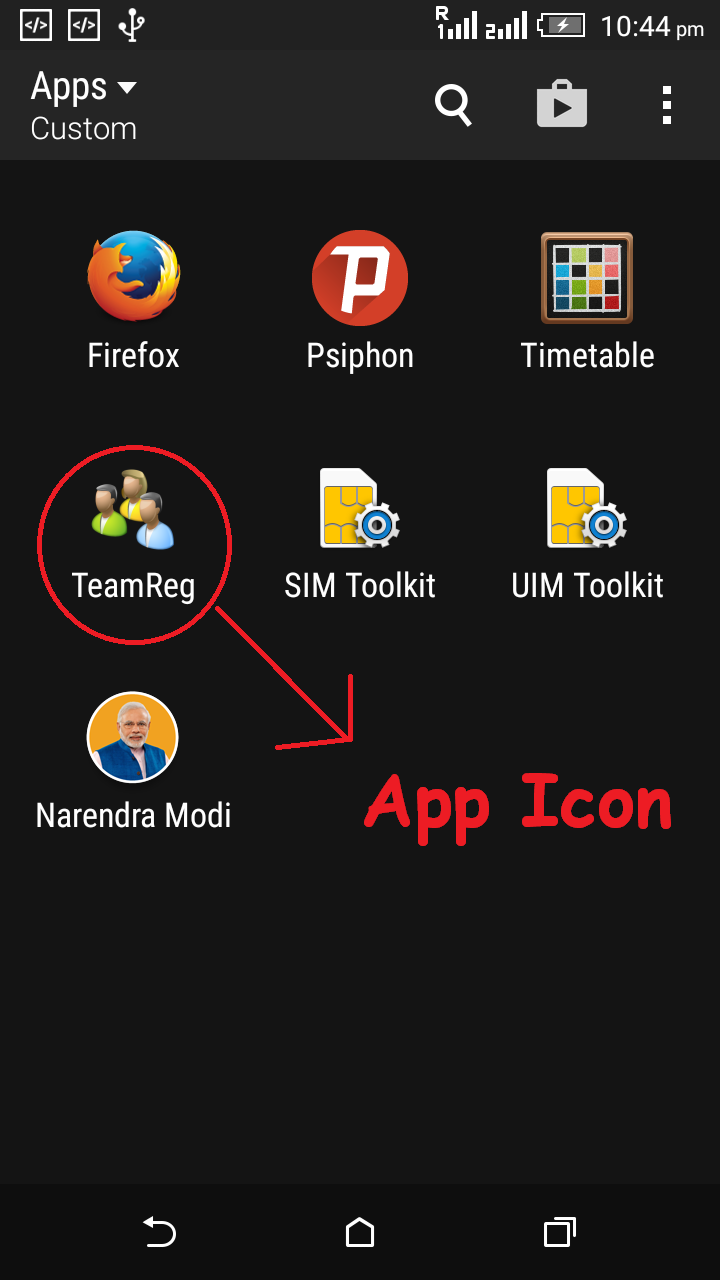
\includegraphics[width=0.5\textwidth]{0.png}
	\caption{App Icon}
\end{figure}

\begin{figure}[!ht]
	\centering
	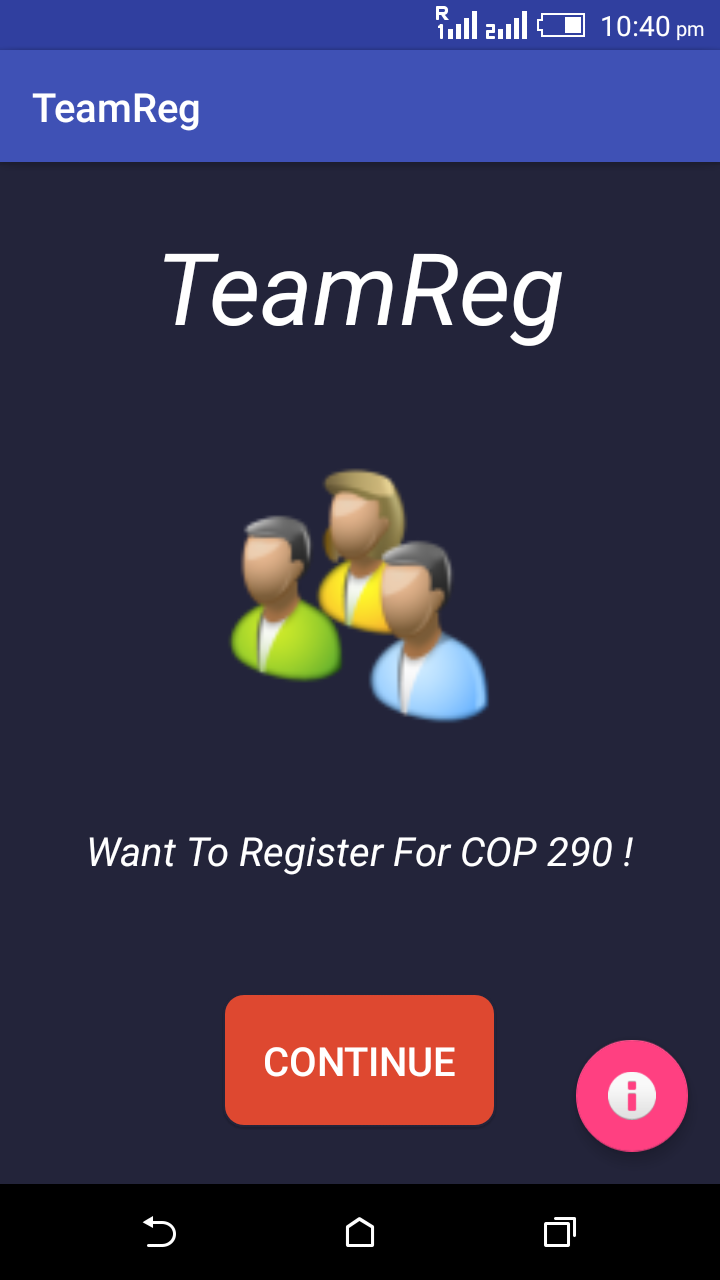
\includegraphics[width=0.5\textwidth]{1.png}
	\caption{Home Screen}
\end{figure}

\begin{figure}[!ht]
	\centering
	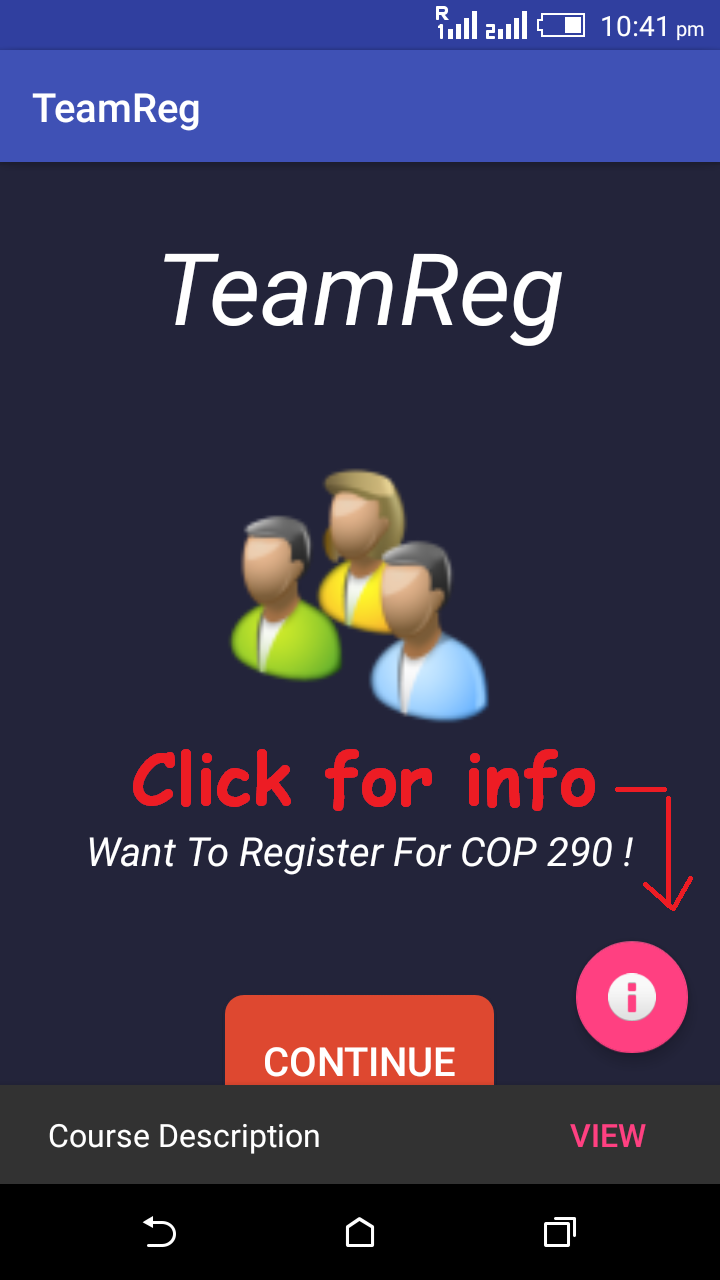
\includegraphics[width=0.5\textwidth]{2.png}
	\caption{Info Button}
\end{figure}

\begin{figure}[!ht]
	\centering
	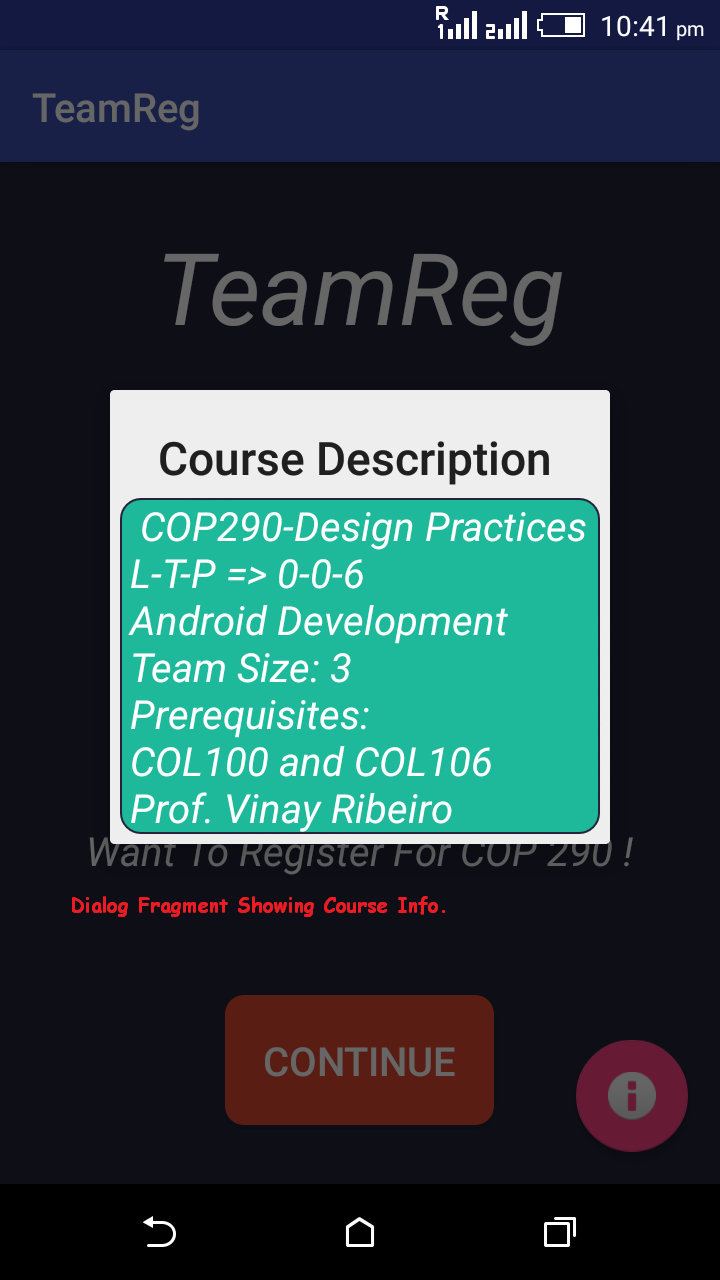
\includegraphics[width=0.5\textwidth]{3.png}
	\caption{Course Description}
\end{figure}

\begin{figure}[!ht]
	\centering
	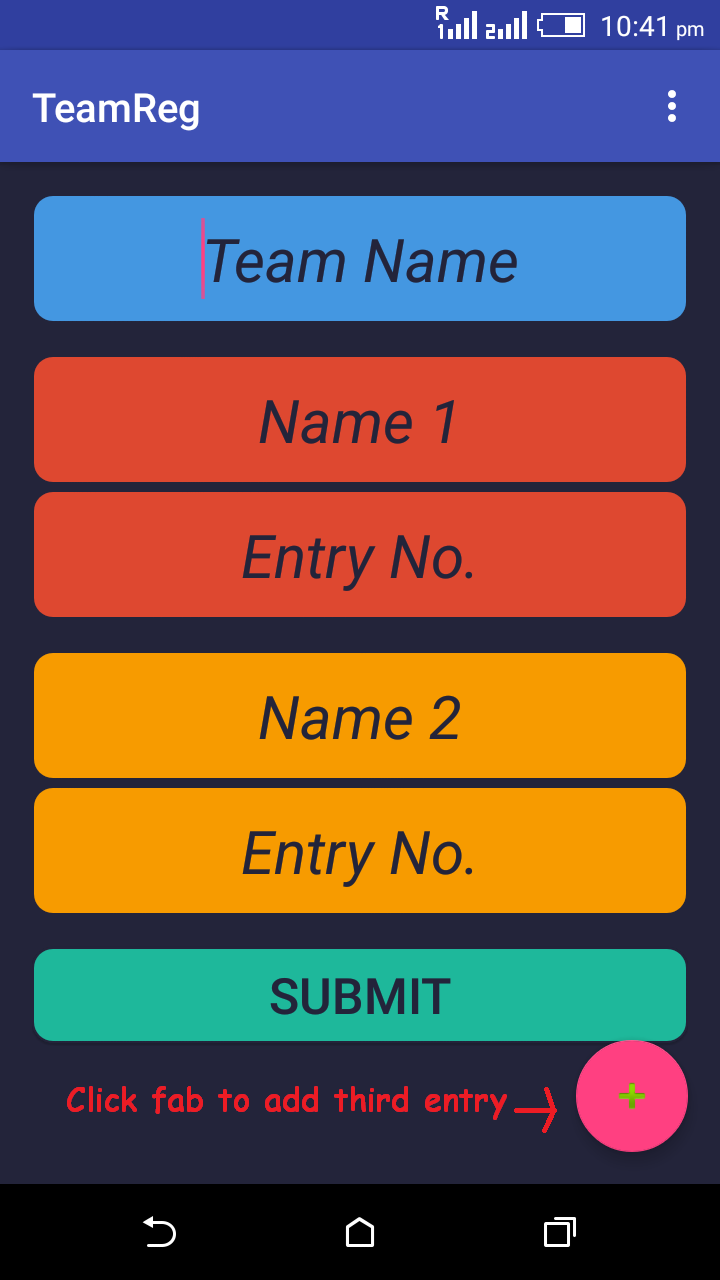
\includegraphics[width=0.5\textwidth]{4.png}
	\caption{Floating Action Add}
\end{figure}

\begin{figure}[!ht]
	\centering
	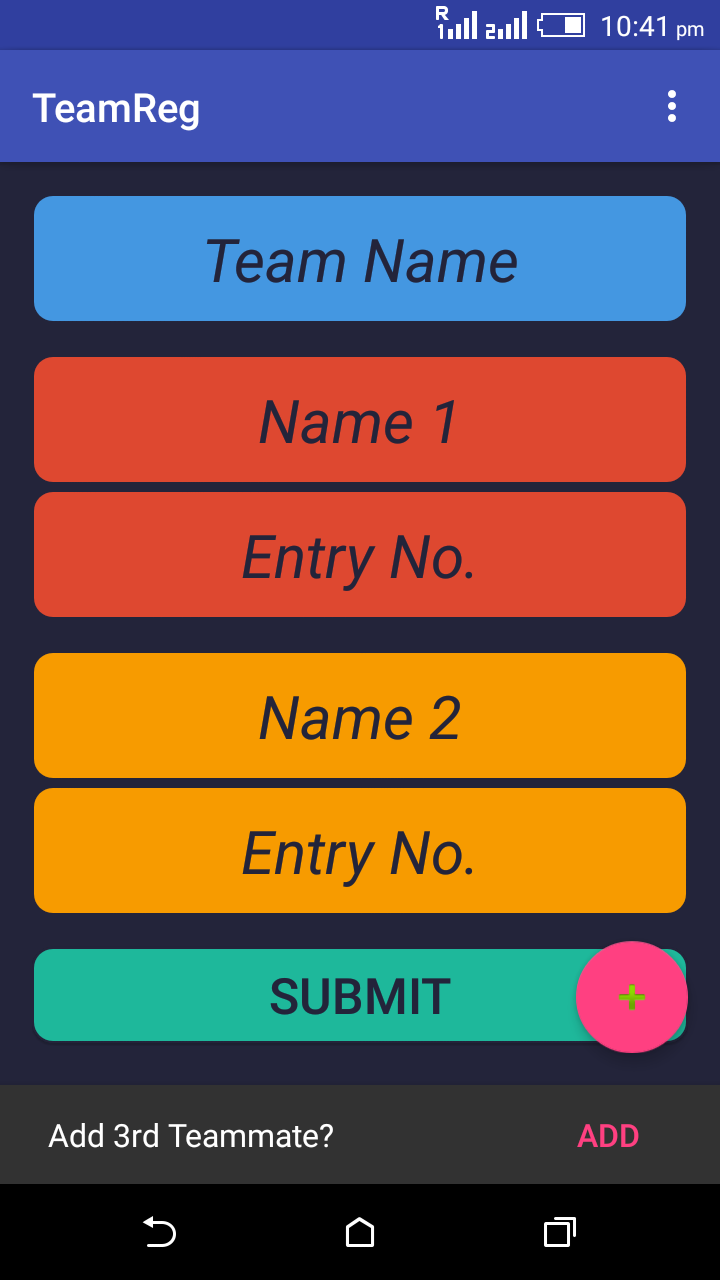
\includegraphics[width=0.5\textwidth]{5.png}
	\caption{Add Entry}
\end{figure}

\begin{figure}[!ht]
	\centering
	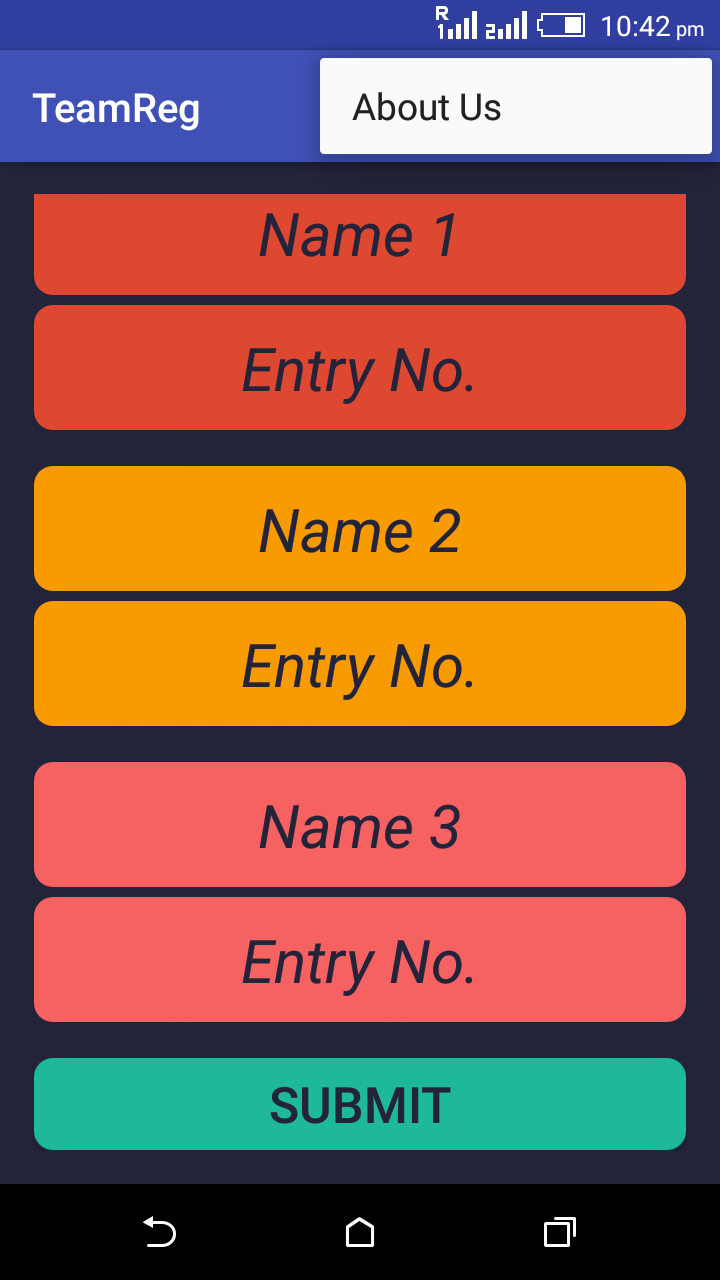
\includegraphics[width=0.5\textwidth]{6.png}
	\caption{Main Menu}
\end{figure}

\begin{figure}[!ht]
	\centering
	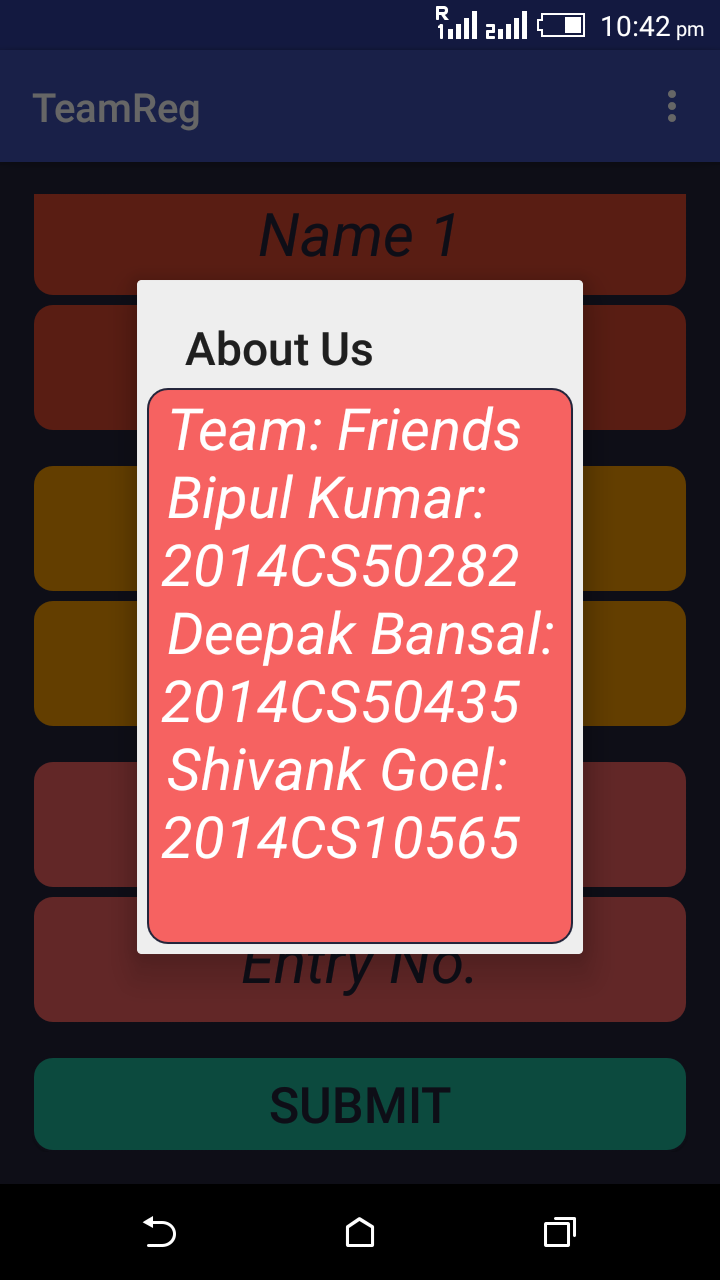
\includegraphics[width=0.5\textwidth]{7.png}
	\caption{About us}
\end{figure}

\end{center}


\begin{itemize}
\item Home Screen
	\begin{itemize}
	\item Home Screen shows a visual layout depicting the aim of the app and providing an option to view the course description before registration.
	\item You can click on fab\cite{android_fab_tutorial} info button to view course description. 
	\item Click Continue to move to the registration page.
	\end{itemize}
\item Registration Screen
	\begin{itemize}
		\item Registration Screen allows you to register for the course. By default it allows two members per team to register for the course.
		\item Clicking add button adds the fields for third member registration.\cite{android_snack_tutorial}
		\item Clicking options menu on appbar displays information about the app authors.\cite{android_diag_tutorial} 
		\item On clicking submit button various toasts are displayed according to current registration status.
	\end{itemize}
\end{itemize}









\section{Implementation Details}

\begin{itemize}
\item We have created two activities in our app 'home activity' and 'main activity' which handle the respective two screens.
\item We have used dialog fragmets to display course description and authors information.
\item We have put all the strings used in strings.xml, all shapes in drawable folder , for better organisation.
\item We have done proper commenting for future reference and collaboration.

\item Methods to verify the user information
	\begin{itemize}
		\item Added a regex to name and entry number column to make sure its a valid entry.
	\end{itemize}
\item Methods for network communication. You can cite material that you used to create the application~\cite{android_network_tutorial}.

\end{itemize}


The code for the project is being maintained in this repository: 
\begin{center}
	 https://github.com/shivankgoel/teamreg.git
\end{center}

\bibliographystyle{abbrv}
\bibliography{references}




\end{document}
